\documentclass[]{report}

\voffset=-1.5cm
\oddsidemargin=0.0cm
\textwidth = 480pt

\usepackage{framed}
\usepackage{subfiles}
\usepackage{enumerate}
\usepackage{graphics}
\usepackage{newlfont}
\usepackage{eurosym}
\usepackage{amsmath,amsthm,amsfonts}
\usepackage{amsmath}
\usepackage{color}
\usepackage{amssymb}
\usepackage{multicol}
\usepackage[dvipsnames]{xcolor}
\usepackage{graphicx}
\begin{document}


HibColl Videos

%% --------------------%% --------------------%% --------------------%% --------------------%% ------------------------

1.A  Converting from Decimal to Binary
1.B  Converting from Decimal to Hexadecimal
1.C  Converting from Binary to Decimal
1.D  Converting from Hexadecimal to Decimal
1.E  Binary Addition
1.F  Binary Subtraction

%% --------------------%% --------------------%% --------------------%% --------------------%% ------------------------

2.A  Membership Tables
2.B  Venn Diagrams
2.C  Set differences and symmetric difference
2.D  
2.E



\chapter{Number Systems}
\subsection{Significant Digits}
There are three rules on determining how many significant figures are in a number: Non-zero digits are always significant. Any zeros between two significant digits are significant. A final zero or trailing zeros in the decimal portion ONLY are significant.

\section{Floating Point Notation}



In computing, floating point describes a method of 
representing an approximation of a real number in a 
way that can support a wide range of values. 


The numbers are, in general, represented approximately 
to a fixed number of significant digits (the mantissa) and scaled using an exponent. 

In essence, computers are integer machines and are capable of representing real numbers only by using complex codes. The most popular code for representing real numbers is called the IEEE Floating-Point Standard .
The term floating point is derived from the fact that there is no fixed number of digits before and after the decimal point; that is, the decimal point can float. There are also representations in 
which the number of digits before and after the decimal point is set, called fixed-point representations. In general, floating-point representations are slower and less accurate than fixed-point representations, but they can handle a larger range of numbers.







\section*{Part A: Number Systems - Binary Numbers}
\begin{enumerate}
\item Express the following decimal numbers as binary numbers.
  \begin{multicols}{4}
    \begin{itemize}
    \item[i)] $(73)_{10}$
    \item[ii)] $(15)_{10}$
    \item[iii)] $(22)_{10}$
    \end{itemize}
  \end{multicols}

  All three answers are among the following options.
  \begin{multicols}{4}
    \begin{itemize}
    \item[a)] $(10110)_{2}$ %22
    \item[b)] $(1111)_{2}$ %15
    \item[c)] $(1001001)_{2}$ %73
    \item[d)] $(1000010)_{2}$ %64
    \end{itemize}
  \end{multicols}

\item Express the following binary numbers as decimal numbers.
  \begin{multicols}{4}
    \begin{itemize}
    \item[a)] $(101010)_{2}$
    \item[b)] $(10101)_{2}$
    \item[c)] $(111010)_{2}$
    \item[d)] $(11010)_{2}$
    \end{itemize}
  \end{multicols}
  \item Express the following binary numbers as decimal numbers.
  \begin{multicols}{4}
    \begin{itemize}
    \item[a)] $(110.10101)_{2}$
    \item[b)] $(101.0111)_{2}$
    \item[c)] $(111.01)_{2}$
    \item[d)] $(110.1101)_{2}$
    \end{itemize}
  \end{multicols}
\item Express the following decimal numbers as binary numbers.
  \begin{multicols}{4}
    \begin{itemize}
    \item[a)] $(27.4375)_{10}$  %
    \item[b)] $(5.625)_{10}$
    \item[c)] $(13.125)_{10}$
    \item[d)] $(11.1875)_{10}$
    \end{itemize}
  \end{multicols}
\end{enumerate}
\newpage
\section*{Part B: Number Systems - Binary Arithmetic}
%http://www.csgnetwork.com/binaddsubcalc.html
%(See section 1.1.3 of the text)
\begin{enumerate}
\item Perform the following binary additions.
  \begin{multicols}{2}
    \begin{itemize}
    \item[a)] $(110101)_{2}$ + $(1010111)_{2}$
    \item[b)] $(1010101)_{2}$ + $(101010)_{2}$
    \item[c)] $(11001010)_{2}$ + $(10110101)_{2}$
    \item[d)] $(1011001)_{2}$ + $(111010)_{2}$
    \end{itemize}
  \end{multicols}

\item Perform the following binary subtractions.
  \begin{multicols}{2}
    \begin{itemize}
    \item[a)] $(110101)_{2}$ - $(1010111)_{2}$
    \item[b)] $(1010101)_{2}$ - $(101010)_{2}$
    \item[c)] $(11001010)_{2}$ - $(10110101)_{2}$
    \item[d)] $(1011001)_{2}$ - $(111010)_{2}$
    \end{itemize}
  \end{multicols}


\item Perform the following binary multiplications.
\begin{multicols}{2}
\begin{itemize}
\item[a)] $(1001)_{2}\times( 1000)_{2}$  % 9 by 8
\item[b)] $(101)_{2}\times(1101)_{2}$ % 5 by 11
\item[c)] $(111)_{2}\times(1111)_{2}$ % 7 by 15
\item[d)] $(10000)_{2}\times(11001)_{2}$    %16 by 25
\end{itemize}
 \end{multicols}



\item Perform the following binary multiplications.
%\begin{multicols}{2}
%\begin{itemize}
%\item[a)] $(1001000)_{2} \div ( 1000)_{2}$
%\item[b)] $(101101)_{2} \div (1001)_{2}$
%\item[c)] $(1001011000)_{2} \div (101000)_{2}$
%\item[d)] $(1100000)_{2} \div (10000)_{2}$
%\end{itemize}
%\end{multicols}

%----------------------------------------------------------------%

\item Perform the following binary divisions.
%\begin{multicols}{2}
%\begin{itemize}
%\item[a)] $(1001000)_{2} \div ( 1000)_{2}$
%\item[b)] $(101101)_{2} \div (1001)_{2}$
%\item[c)] $(1001011000)_{2} \div (101000)_{2}$
%\item[d)] $(1100000)_{2} \div (10000)_{2}$
%\end{itemize}
%\end{multicols}


% \newpage
\section*{Part D: Natural, Rational and Real Numbers}
\begin{framed}
\begin{itemize}
\item $\mathbb{N}$ : natural numbers (or positive integers) $\{1,2,3,\ldots\}$
\item $\mathbb{Z}$ : integers $\{-3,-2,-1,0,1,2,3,\ldots\}$
\begin{itemize}
\item[$\ast$] (The letter $\mathbb{Z}$ comes from the word \emph{Zahlen} which means ``numbers" in German.)
\end{itemize}
\item $\mathbb{Q}$ : rational numbers
\item $\mathbb{R}$ : real numbers
\item $\mathbb{N} \subseteq \mathbb{Z } \subseteq \mathbb{Q} \subseteq \mathbb{R}$
\begin{itemize}
\item[$\ast$] (All natural numbers are integers. All integers are rational numbers. All rational numbers are real numbers.)
\end{itemize}
\end{itemize}
\end{framed}

\begin{enumerate}
\item State which of the following sets the following numbers belong to. 
  \begin{multicols}{4}
    \begin{itemize}
    \item[1)] $18$
    \item[2)] $8.2347\ldots$
    \item[3)] $\pi$
    \item[4)] $1.33333\ldots$
    \item[5)] $17/4$
    \item[6)] $4.25$
    \item[7)] $\sqrt{\pi}$
    \item[8)] $\sqrt{25}$
    %\item[i)]
    %\item[j)] $(15)_{10}$
    %\item[k)] $\pi$
    %\item[l)] $11.132$
    \end{itemize}
  \end{multicols}
  \bigskip
  The possible answers are

    \begin{itemize}
    \item[a)] Natural number : $\mathbb{N} \subseteq \mathbb{Z } \subseteq \mathbb{Q} \subseteq \mathbb{R}$
    \item[b)] Integer : $ \mathbb{Z } \subseteq \mathbb{Q} \subseteq \mathbb{R}$
    \item[c)] Rational Number : $ \mathbb{Q} \subseteq \mathbb{R}$
    \item[d)] Real Number $\mathbb{R}$

    %\item[i)]
    %\item[j)] $(15)_{10}$
    %\item[k)] $\pi$
    %\item[l)] $11.132$
    \end{itemize}

\end{enumerate}


% \item The Fibonacci sequence $f_n$ is defined recursively by the rule
%   \begin{equation*}
%     \begin{cases}
%       f_0&=0\\
%       f_1&=1\\
%       f_n&=a_{n-1}+a_{n-2}
%     \end{cases}
%   \end{equation*}

%   \begin{enumerate}
%   \item
%     Write a program to evaluate the Fibonacci sequence and hence evaluate $f_{50}$.
%   \item
%     Let the sequence $g_n$ be defined as the ratio
%     \begin{equation*}
%       g_n = \frac{f_{n+1}}{f_n}
%     \end{equation*}
%     Write a program to evaluate the first $50$ terms of the sequence $g_n$.
%   \item
%     Assumming that the sequence $g_n$ has a limit $\phi$, find this limit.
%   \end{enumerate}


\subsection*{Floating Point Notation}
(Demonstration on white board)






% \newpage
\section*{Part D: Natural, Rational and Real Numbers}
\begin{itemize}
\item $\mathbb{N}$ : natural numbers (or positive integers) $\{1,2,3,\ldots\}$
\item $\mathbb{Z}$ : integers $\{-3,-2,-1,0,1,2,3,\ldots\}$
\begin{itemize}
\item (The letter $\mathbb{Z}$ comes from the word \emph{Zahlen} which means ``numbers" in German.)
\end{itemize}
\item $\mathbb{Q}$ : rational numbers
\item $\mathbb{R}$ : real numbers
\item $\mathbb{N} \subseteq \mathbb{Z } \subseteq \mathbb{Q} \subseteq \mathbb{R}$
\begin{itemize}
\item (All natural numbers are integers. All integers are rational numbers. All rational numbers are real numbers.)
\end{itemize}
\end{itemize}




\subsection{Irrational Numbers}
An irrational number cannot be expressed as a ratio between two numbers and it cannot be written as a simple fraction because there is not a finite number of numbers when written as a decimal. Instead, the numbers in the decimal would go on forever, without repeating.



In mathematics, the cardinality of a set is a measure of the "number of elements of the set". For example, the set A = {2, 4, 6} contains 3 elements, and therefore A has a cardinality of 3.





\chapter{Set Theory}



\section{Set Theory}
\begin{enumerate}
\item The Universal Set $\mathcal{U}$
\item Union
\item Intersection
\item Set Difference
\item Relative Difference
\end{enumerate}

\newpage


NOTATIONS FOR A SET:

A set can be represented by two methods:
1.ROSTER METHOD
2.BUILDER METHOD
ROSTER METHOD:

In this method the elements of a set are separated by commas and are enclosed within curly brackets { }. For example:

$A = {1, 2, 3, 4, 5, 6}$ is a set of numbers.

B = {Sunny, Joy, Kartik, Harish, Girish} is a set of names.

C = {a, e, i, o, u} is a set of vowels.

D = {apple, banana, guava, orange, pear} is a set of fruits.

Listing the elements in this way is called Roster method. In this method, it is not necessary for the elements to be listed in a particular order. The elements of the set can be written just plainly, separated by commas and in any order.


BUILDER METHOD:

This method is also called Property method. In Builder method, a set is represented by stating all the properties which are satisfied by the elements of that particular set only.

For example:

If A is a set of elements less than 0, then in Builder method it will be written as

$A = {x: x < 0}$, this statement is read as "the set of all x such that x is less than 0"

If A is a set of all real numbers less than 7, then in Builder method it is written as $A = {x   R: x < 7}$

Similarly,

$A = {2i: i is an integer}$ is a set of all even integers.

$A = {x   R: x \neq 2}$ is a set of all real numbers except 2.

$A = {x   R: x > 3 and x < 7}$ is a set of real numbers greater than 3 but less than 7.

$A = {x   Z: x > 6}$ is a set of integers greater than 6.

$A = {x   Z: 2x + 1}$ is a set of all odd integers.


\subsection{Proper subset definition.} 
A proper subset of a set A is a subset of A that is not equal to A. In other words, if B is a proper subset of A, then all elements of B are in A but A contains at least one element that is not in B. For example, if A={1,3,5} then B={1,5} is a proper subset of A.



%---------------------------------------%


%%- Question 2B 2010 Zone A


\begin{itemize}
\item Let A and B be subsets of the a universal set $U$.
\item Use membership tables to prove that $(A \cup B^{\prime})^{\prime}$ = $A^{\prime} \cap B$
\item Shade the regions corresponding to this set on a Venn Diagram
\end{itemize}

\begin{tabular}{|c|c|| c | c| c|}
A&B&$B^{\prime}$&$A \cup B^{\prime}$&$(A \cup B^{\prime})^{\prime}$\\ \hline
0&0&1&1&0\\
0&1&0&0&1\\
1&0&1&1&0\\
1&1&0&1&0\\
\end{tabular}

\begin{tabular}{|c|c|| c | c| }
A&B&$A^{\prime}$&$A^{\prime} \cap B$\\\hline
0&0&1&0\\
0&1&1&1\\
1&0&0&0\\
1&1&0&0\\
\end{tabular}



%-------------------------------------------%
% 2010 Zone A Q 1c
Given the universal set $U$ and subsets $A$ and $B$, list the set $(A \cup B^{\prime})^{\prime}$
\begin{itemize}
\item $U=\{1,2,\ldots,8,9\}$
\item $A=\{2,4,6,8\}$
\item $B=\{ 4,5,6,7\}$
\item $B^{\prime}=\{ 1, 2, 3, 8, 9  \}$
\item $A \cup B^{\prime}=\{ 1, 2, 3,4, 6, 8, 9  \}$
\item $(A \cup B^{\prime})^{\prime}=\{ 5,7 \}$
\end{itemize}




%----------------------------------------------------------------%

\subsection{Number Sets}

%% %% - \vspace{-1cm}
\textbf{Blackboard Bold Typeface}

\begin{itemize}
\item Conventionally the symbols for numbers sets are written in a special typeface, known as \textbf{blackboard bold}.
\item Examples : $\mathbb{N}$, $\mathbb{Z}$ and $\mathbb{R}$.

\end{itemize}


%% %% - \vspace{-1cm}
\textbf{Natural Numbers} ($\mathbb{N}$)
\begin{itemize}
\item The whole numbers from 1 upwards. 

\item The set of natural numbers is 
\[\{1,2,3,4,5,6,\ldots\} \]
\item In some branches of mathematics, $0$ might be counted as a natural number.
\[\{0,1,2,3,4,5,6,\ldots\} \]
\end{itemize}

%----------------------------------------------------------------%


\subsection{Number Sets}


%% %% - \vspace{-0.5cm}
\textbf{Integers} ($\mathbb{Z}$)
\begin{itemize}
\item The integers are all the whole numbers, all the negative whole numbers and zero.

\item The set of integers is 
\[\{\ldots,-4,-3,-2,-1,\;0,\;1,\;2,\;3,\ldots\} \]
\item The notation $\mathbb{Z}$ is from the German word for numbers: \textit{Zahlen}. 
\item All natural numbers are integers.
\[ \mathbb{Q}  \subset \mathbb{Z}\]
\end{itemize}

%----------------------------------------------------------------%


\subsection{Number Sets}

%% %% - \vspace{-1.8cm}
\textbf{Integers} ($\mathbb{Z}$)
\begin{itemize}
\item Natural numbers may also be referred to as positive integers, denoted $\mathbb{Z}^{+}$. \\(note the superscript)
\item Negative integers are denoted $\mathbb{Z}^{-}$.
\[\{\ldots,-4,-3,-2,-1\}\]
\end{itemize}

%----------------------------------------------------------------%


\subsection{Number Sets}

%% %% - \vspace{-1.8cm}
\textbf{Integers} ($\mathbb{Z}$)
\begin{itemize}
\item 0 is neither positive nor negative. The following set of non-negative numbers \[\{0,1,2,3,4,5,6,\ldots\} \] might be denoted $0 \cup \mathbb{Z}^{+}$
\item $\cup$ is the mathematical symbol for \textbf{union}.
\end{itemize}



\subsection{Number Sets}

%% %% - \vspace{-1cm}
\textbf{Rational Numbers} ($\mathbb{Q}$)
\begin{itemize}
\item Rational numbers, also known as quotients, are numbers you can make by dividing one integer by another (but not dividing by zero). 
\item If a number can be expressed as one integer divided by another, it is a rational number.
\[ \mathbb{Q} = \left\{\; \frac{p}{q} \;\bigg| p \in \mathbb{Z},\; q \in \mathbb{Z},\; q \neq 0  \;   \right\}   \]
\end{itemize}

%-------------------------------------------------------------- %   

\subsection{Number Sets}

%% %% - \vspace{-1cm}
\textbf{Rational Numbers} ($\mathbb{Q}$)
\begin{itemize}
\item All integers are rational numbers 
\[ \mathbb{Z}  \subset \mathbb{Q}\]
(and by extension all natural numbers are rational numbers too)
\item Examples of rational numbers
\[ 9500,\;7,\; \frac{1}{2} ,\; \frac{3}{7},\; -2.6 ,\; 0.001\] 
\end{itemize}

%-------------------------------------------------------------- %   

\subsection{Number Sets}

%% %% - \vspace{-1cm}
\textbf{Irrational Numbers} 
\begin{itemize}
\item A number that can not be written as the ratio of two integers is known as an irrational number.
\item Two famous examples of irrational numbers are $\pi$ and $\sqrt{2}$. 
\[\pi = 3.141592\ldots\]
\[\sqrt{2} = 1.41421\ldots\]
\end{itemize}


%% %% - \vspace{-1cm}
\textbf{Real Numbers} ($\mathbb{R}$)
\begin{itemize}
\item Irrational numbers are types of real numbers.
\item Rational numbers are real numbers too.
\[ \mathbb{Q}  \subset \mathbb{R}\]

\item A real number is simply any point anywhere on the number line.
\end{itemize}


%% %% - \vspace{-1cm}
\textbf{Real Numbers} ($\mathbb{R}$)
\begin{itemize}
\item There are numbers that are not real numbers, for example \textbf{imaginary numbers}, but we will not cover them in this presentation.
\end{itemize}


%------------------------------------------$
2010 Zone B Q 1

5n+1 Rules of Inclusion method

$A = \{5n+1: n \in Z \}$

\subsection*{2011 Zone A question 1d}

Showing your workings, express the repeating decimal 0.012012012012...
as a rational number in its simplest form.


\begin{itemize}
\item x = 0.012012012012...
\item 10x = 0.12012012012... (not particularly useful )
\item 100x = 1.2012012012... (not particularly useful either)
\item 1000x= 12.012012012... (very useful)
\item 999x = 12
\item x= 12/999 = 4/333 (Answer!)
\end{itemize}

\chapter{graph theory }
Given the following definitions for simple, connected graphs:
\begin{itemize}
\item $K_n$ is a graph on $n$ vertices where each pair of vertices is connected by an edge;
\item $C_n$ is the graph with vertices $v_1, v_2, v_3, \dots, v_n$ and edges $\{v_1,v_2\}, \{v_2,v_3\}, \dots\{v_n, v_1\}$;
\item $W_n$ is the graph obtained from $C_n$ by adding an extra vertex,$v_{n+1}$, and edges
from this to each of the original vertices in $C_n$.
\end{itemize}
(a) Draw $K_4$, $C_4$, and $W_4$. 
%%% --------------------%% --------------------%% --------------------%% --------------------%% --------------------%% --------------------%% --------------------%% --------------------%% --------------------%% ------------------------%


\section{Set Theory}
\begin{enumerate}
\item The Universal Set $\mathcal{U}$
\item Union
\item Intersection
\item Set Difference
\item Relative Difference
\end{enumerate}



DE Muorgan's Laws (Useful for Propositions)

membership tables

proof by truth tables
AND
OR
NOT
Set difference
symmetric difference



\newpage


Harmonic Mean

\[ H_x = \frac{ n }{ \frac{ 1 }{ x_1 } + \frac{ 1 }{ x_2 } + \cdots + \frac{ 1 }{ x_n } } \]

2,4,6,8
> 1/mean(1/a)
[1] 3.84
> 1/a
[1] 0.5000000 0.2500000 0.1666667 0.1250000
> sum(1/a)
[1] 1.041667
> sum(1/a)*24
[1] 25
> 96/25
[1] 3.84



\subsection{Functions}
Consider the floor function $f : R \rightarrow Z$ given the rule

\[ f(x) = \lfloor \frac{x+1}{2} \rfloor \]

\begin{enumerate}
\item evaluate $f(6)$ and $f(-6)$
\item Show that f(x) is not one-to-one
\item 
\end{enumerate}

%----------------------------------------%

\subsection{Functions}
Evaluate $f(6)$ 


\[ f(x) = \lfloor \frac{x+1}{2} \rfloor \]


\[ f(6) = \lfloor \frac{\boldsymbol{6}+1}{2}\rfloor = \lfloor  \frac{7}{2}\rfloor\]


\[  \lfloor 3.5 \rfloor  = 3  \]


%----------------------------------------%

\subsection{Functions}
Evaluate $f(-6)$ 


\[ f(x) = \lfloor \frac{x+1}{2} \rfloor \]


\[ f(6) = \lfloor \frac{\boldsymbol{-6}+1}{2}\rfloor = \lfloor  \frac{-5}{2}\rfloor\]


\[  \lfloor -2.5 \rfloor  = -3  \]






% http://www.textbooksonline.tn.nic.in/books/12/std12-bm-em-1.pdf


\subsection{Discrete Maths : Relations}

\begin{itemize}
\item A relation $R$ from a set A to a set B is a subset of the
\textbf{cartesian product} A x B. 
\item Thus R is a set of \textbf{ordered pairs} where
the first element comes from A and the second element comes
from B i.e. $(a, b)$
\end{itemize}

%-----------------------------------%

\subsection{Discrete Maths : Relations}

\begin{itemize}

\item  If $(a, b) \in R$ we say that $a$ is related to $b$ and write $aRb$.
\item If $(a, b) \notin R$, we say that $a$ is not related to $b$ and write $aRb$. CHECK
\item If
$R$ is a relation from a set $A$ to itself then we say that ``$R$ is a relation
on $A$".
\end{itemize}

%-----------------------------------%

\subsection{Discrete Maths : Relations}

%% %% - \vspace{-2cm}
\textbf{Example}
\begin{itemize}
\item Let $A = \{2, 3, 4, 6\}$ and $B = \{4, 6, 9\}$
\item Let R be the relation from A to B defined by \textit{\textbf{xRy}} if $x$
divides $y$ exactly.
\end{itemize}


%-----------------------------------%

\subsection{Discrete Maths : Relations}

%% %% - \vspace{-0.7cm}
\textbf{Example}
\begin{itemize}

\item Let $A = \{2, 3, 4, 6\}$ and $B = \{4, 6, 9\}$
\item Let R be the relation from A to B defined by \textit{\textbf{xRy}} if $x$
divides $y$ exactly.
\item  Then
\[R = {(2, 4), (2, 6), (3, 6), (3, 9), (4, 4), (6, 6)}\]
\end{itemize}



%------------------------------------------------------------------------%
\section{Arrow Diagrams}

\begin{itemize}

\item Domain
\item Co-Domain
\item Range
\end{itemize}
\[  f(x) : \mbox{Domain} \rightarrow \mbox{Co-Domain} \]
\[  f(x) : \mathbb{R} \rightarrow \mathbb{R} \]
%----------------------------------------------------------- %
\newpage
\subsection*{Polynomial Functions (4.1.5)}

\begin{itemize}
\item[Constants] $(P_0)$
\item[Linear Functions] $(P_1)$
\item[Quadratic Functions] $(P_2)$
\item[Cubic Functions] $(P_3)$
\end{itemize}


\subsection*{Equality of Functions (4.1.6)}
\[f(x) = g(x) \]




%------------------------------------------------------%
\subsection{Exercise} 
$h(x): \mathbb{R} \rightarrow \mathbb{R}$ 
$g(x): \mathbb{R} \rightarrow \mathbb{R}$

\[f(x) = sqrt(x)\]
\[g(x) = \sqrt{3}{x+2}\]
\[h(x) = 2^x\]

\begin{itemize}
\item Is the function $h(x)$ an \textit{onto} function?
\item determine the inverse function of $h(x)$ and $g(x)$
\item Simplify the following function.
\[ j(x) = \mbox{log}_4(h(6x))\]
\end{itemize}
%--------------------------------------------%
\subsection{Onto Functions}
Definition: If every element in the co-domain of the function has an ancestor, the function is said to be "onto".
An onto function has the property that the domain is equal to the co-domain.


\textbf{Example 4.26 Page 53}

%------------------------------------------------------------------------%
\section{\textit{One-to-One} Functions and \textit{Onto} Functions}

\subsection{Invertible Functions}
\begin{itemize}
\item One-to-One Function
\item Onto Function
\end{itemize}

Onto Functions : Range and Co-Domain are equivalent

\subsection{Inverting a Function}

\begin{itemize}
\item[$\bullet$] You are given $f(x)$ in terms of $x$
\item[$\bullet$] Re-arrange the equation so that $x$ is given in terms of $f(x)$
\item[$\bullet$] Replace $x$ with $f^{-1}(x)$ and $f(x)$ with $x$
\end{itemize}

\subsubsection{Example}
\begin{itemize}
\item[$\bullet$]Determine the inverse function of $f(x)$. Re-arrange the equation so that $x$ is given in terms of $f(x)$
\[  f(x): \mathbb{R} \rightarrow \mathbb{R}  \mbox{   } f(x)  = \sqrt{x+1} \]
\item[$\bullet$] Square both sides of the equation.
\[[f(x)]^2 = x+1 \]
\item[$\bullet$] Subtract 1 from both sides of the equation. We have the equation written in terms of x.
\[f(x)^2-1 = x \]
\item[$\bullet$] Replace $x$ with $f^{-1}(x)$ and $f(x)$ with $x$
\[x^2-1 = f^{-1}(x) \]
\item[$\bullet$] 
Re-arrange equation and specify domain and co-domain.
\[ f(x): \mathbb{R} \rightarrow \mathbb{R}  \mbox{   }  f^{-1}(x) = x^2-1  \]
\end{itemize}
% \[ f(x)  = \sqrt{x+1} \]
% \[f(x)^2 = x+1 \]
% \[f(x)^2-1 = x \]
% \[x^2-1 = f^{-1}(x) \]
\newpage
\section{Big O-Notation}

%------------------------------------------------------------------------%
% Section 4 Functions
% http://doc.gold.ac.uk/~maa01km/solutions/tut4sol.pdf

\item[(b)] Let $S$ be the set of all 4 bit binary strings. 

The function $f : S \rightarrow \mathbb{Z}$
is defined by the rule:
\[f(x) = \mbox{the number of zeros in x}\]
for each binary string $x \in S$.\\
Find:
\begin{enumerate}
\item the number of elements in the domain
\item $f(1000)$
\item the set of pre-images of 1
\item the range of $f$.
\end{enumerate}
\item[(c)]
\end{itemize}
\newpage
\begin{itemize}
\item[4.a] $ \lfloor x - y \rfloor = \lfloor x \rfloor - \lfloor y \rfloor$
\item[4.b]
\item[4.c]
\end{itemize}
\newpage
%------------------------------------------------------------------------%
\section{Section 4 Functions}

\subsection{Invertible Functions}
A function is invertible if it fulfils two criteria
\begin{itemize}
\item The function is \textbf{\textit{onto}},
\item The function is \textbf{\textit{one-to-one}}.
\end{itemize}

State the conditions to be satisfied by a function
$f : X \leftarrow Y$ for it to have an inverse function
$f^{-1} : Y \leftarrow X$.
%---------------------------------------------------------%

$\lceil \frac{x^2+1}{4} \rceil$
where $f : A \rightarrow \textbf{Z}$
\begin{itemize}
\item[(i)] Find $f(4)$ and the ancestors of 3.
\item[(ii)] Find the range of $f$.
\item[(iii)] Is f invertible? Justify your answer
\end{itemize}

Given $f : \textbf{R} \rightarrow \textbf{R}$ where f(x) =3x-1,define fully
the inverse of the function f ,i.e.$f^{-1}$. 
State the value of $f^{-1}(2)$


\newpage

\section*{Prepositional Logic}

\subsection{five basic connectives}


%--------------------------------------------------%
Reflexive, Symmetric and Transitive

\begin{itemize} 
\item Reflexive
\item Symmetric
\item Transitive
\end{itemize}

%--------------------------------------------------%
\subsection{Logarithms}


Here we
assume x and y are positive real numbers.
1. $loga(xy) = loga(x) + loga(y)$
2. $loga(x/y)= loga(x) - loga(y)$
3. $loga (x^r) = r loga(x)$ for any real number r.
%--------------------------------------------------%
Invertible Functions

%--------------------------------------------------%
\subsection{Proof by Induction}

Another sequence is defined by the recurrence relation un = un-1+2n-1 and
u1 = 1.
(i) Calculate u2, u3, u4 and u5.
1,4,9,16,25

(ii) Prove by induction that $u_n = n^2$ for all $n \geq 1$

%--------------------------------------------------%
Exponentials
% http://www.mathsisfun.com/algebra/exponent-laws.html

\section{Laws of Exponents}
Here are the Laws (explanations follow):

LawExample
x1 = x61 = 6
x0 = 170 = 1
x-1 = 1/x4-1 = 1/4
xmxn = xm+nx2x3 = x2+3 = x5
xm/xn = xm-nx6/x2 = x6-2 = x4
(xm)n = xmn(x2)3 = x2×3 = x6
(xy)n = xnyn(xy)3 = x3y3
(x/y)n = xn/yn(x/y)2 = x2 / y2
x-n = 1/xnx-3 = 1/x3
%--------------------------------------------------%
Z Score
\[ Z = \frac{X - \mu}{\sigma} \]
%--------------------------------------------------%




%-------------------------------------------------------%


%% --------------------
\subsection{Exercises}

Showing your workings, use the rules of indices and logarithms to give the following two expression in their simplest form.
\bigskip
\begin{itemize}
\item \textbf{Exercise 1}
\[ 4 \cdot 2^x - 2^{x+1} \]
\item \textbf{Exercise 2}
\[  \frac{\mbox{ln}(2) + \mbox{ln}(2^2) + \mbox{ln}(2^3)  + \mbox{ln}(2^4) + \mbox{ln}(2^5)  }  {\mbox{ln}(4)}  \]
\end{itemize}
%% --------------------

%-------------------------------------------------------%
%% --------------------
\subsection{Exercise 1}

\[ 4 \cdot 2^x - 2^{x+1} \]

\textbf{Remarks:}\\
\textit{(looking at the second term)}
\begin{itemize}
\item[1] Using the following rule
\[ a^b \cdot a^c = a^{(b+c)}  \] 
\item[2] Using this rule in reverse we can say
\[ 2^{x+1} = 2^x \cdot 2^1  = 2\cdot (2^x) \] 
\end{itemize}
\[ 4 \cdot 2^x - 2^{x+1} \mbox{   } = \mbox{   } (4 \cdot 2^x) -  (2\cdot 2^{x}) \]
%% --------------------

%-------------------------------------------------------%
%% --------------------
\subsection{Exercise 1}

%% %% - \vspace{-0.9cm}

\textbf{Remarks:}
\begin{itemize}
\item[3] This expression is in the form 
\[ (a  \cdot b ) - ( c  \cdot b) \]
which can be re-expressed as follows 
\[ (a - c\sqrt{b} )  \cdot b \]
\end{itemize}
\[ (4 \cdot 2^x) -  (2\cdot 2^{x}) = (4-2)  \cdot 2^{x} \]
\[   = 2 \cdot 2^x = 2^{x+1}\]
%% --------------------
%-------------------------------------------------------%

%% --------------------
\subsection{Exercise 2}


\[  \frac{\mbox{ln}(2) + \mbox{ln}(2^2) + \mbox{ln}(2^3)  + \mbox{ln}(2^4) + \mbox{ln}(2^5)  }  {\mbox{ln}(4)}  \]
Useful Rule of Logarithms
\[  \mbox{ln}(a^b)  = b\cdot \mbox{ln}(a)  \]
\[  \frac{\mbox{ln}(2) + 2 \cdot \mbox{ln}(2) + 3 \cdot\mbox{ln}(2)  + 4 \cdot \mbox{ln}(2) + 5 \cdot \mbox{ln}(2)  }  {\mbox{ln}(4)}  \]
%% --------------------
%--------------------------------------%
%% --------------------
\subsection{Exercise 2}

Adding up all the terms in the numerator

\[  \frac{1\cdot\mbox{ln}(2) + 2 \cdot \mbox{ln}(2) + 3 \cdot\mbox{ln}(2)  + 4 \cdot \mbox{ln}(2) + 5 \cdot \mbox{ln}(2)  }  {\mbox{ln}(4)} \]  \[= \frac{15 \cdot \mbox{ln}(2) }{\mbox{ln}(4)} \]


%% --------------------

%--------------------------------------%
%% --------------------
\subsection{Exercise 2}

Our expression has now simplified to 
\[\frac{15 \cdot \mbox{ln}(2) }{\mbox{ln}(4)} \]

We can simplify the denominator too

\[ \mbox{ln}(4) =  \mbox{ln}(2^2) = 2 \cdot \mbox{ln}(2) \]


%% --------------------

%--------------------------------------%
%% --------------------
\subsection{Exercise 2}

Our expression has now simplified to 
\[\frac{15 \cdot \mbox{ln}(2) }{\mbox{ln}(4)} = \frac{15 \cdot \mbox{ln}(2) }{2 \cdot \mbox{ln}(2)} \]

We can divide above and below by $\mbox{ln}(2)$ to get our final answer


\[ \frac{15 \cdot \mbox{ln}(2) }{2 \cdot \mbox{ln}(2)} = \frac{15}{2} = 7.5 \]

%% --------------------

%% --------------------
%-----------------------------------------------------%
\section*{Prepositional Logic}


%-------------------------------------------------------------------------%
\newpage
\section{Section 3 Logic}
\subsection{Logical Operations}
\begin{itemize}
\item $\neg p$ the negation of proposition $p$.
\item $p \wedge q$ Both propositions p and q are simultaneously true (Logical State AND)
\item $p \vee q $ One of the propositions is true, or both (Logical State : OR)
\item $p \otimes q$ Only one of the propositions is true (Logical State : exclusive OR (i.e XOR)
\end{itemize}
\begin{center}
\begin{tabular}{|c|c|c|c|c|}
\hline
p & q & $p \vee q$ & $q \wedge p$ & $p \otimes q$ \\
\hline
0 & 0 & 0 & 0 & 0 \\
0 & 1 & 1 & 0 & 1\\
1 & 0 & 1 & 0 & 1 \\
1 & 1 & 1 & 1 & 0\\
\hline
\end{tabular}
\end{center}
%---------------------------------------------------------%
\section{Conditional Connectives}
Construct the truth table for the proposition $p \rightarrow q$.

\begin{center}
\begin{tabular}{|c|c|c|c|}
\hline
p & q & $p \rightarrow q$ & $q \rightarrow p$ \\
\hline
0 & 0 & 1& 1 \\
0 & 1 & 1 & 0 \\
1 & 0 & 0 & 1 \\
1 & 1 & 1 & 1 \\
\hline
\end{tabular}
\end{center}

% Question 1 - numbers - Started
% Question 2 - Sets - Not Started
% Question 3 - Logic - Not Started
% Question 4 - Functions - Started
% Question 5 - Graphs
% Question 6 - Digraphs and Relations
% Question 7 - 
% Question 8 -
% Question 9
% Question 10 - Matrices - STARTED

\subsection*{Question 4}
%2001 Question 4
\begin{center}
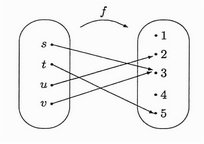
\includegraphics[scale=0.55]{HibCollArrow.jpg}
\end{center}

%---------------------------------------%
\subsection*{Question 6}
%2002 Question 7
Let $\mathcal{S}$ be a set and let $\mathcal{R}$ be a relation on $\mathcal{S}$
Explain what it means to say that $\mathcal{R}$ is

\begin{itemize}
\item[(i)] reflexive
\item[(ii)] symmetrix
\item[(iii)] anti-symmetric
\item[(iv)] Transitive
\end{itemize}


\subsection*{Question 10}

(a) Given the following adjacency matrices A and B where
%A =
%
%1 0 1
%0 1 2
%1 2 0
%
% ,B =
%
%1 2 0
%2 0 1
%0 1 1

%MAKE NO

%--------------------------------------------%

(i) Say whether or not the graphs they represent are isomorphic.
(ii) Calculate A2 and A4 and say what information each gives about the graph
corresponding to A. [6]
(b) (i) Write down the augmented matrix for the following system of equations.

\[2x + y - z = 2\]
\[x - y + z = 4\]
\[x + 2y + 2z = 10\]
(ii) Use Gaussian elimination to solve the system. [4]



\subsection*{Dice Rolls}
Consider rolls of a die. What is the universal set?

\[ \mathcal{U} = \{1,2,3,4,5,6\} \]

%--------------------------------------%

\subsection*{symbols}
$\varnothing$,
$\forall$,
$\in$,
$\notin$,
$\cup$
%----------------------------------------------------------- %
\newpage

\section*{Prepositional Logic}


%-------------------------------------------------------------- %
\begin{itemize}
\item $p \wedge q$
\item $p \vee q$
\item $p \rightarrow q$
\end{itemize}
\newpage
\chapter{Sequences and Series, and Proof by Induction}
\section{Sequence and Series and Proof by Induction}


\[\sum (n^2) \]



\subsection*{Part D : Real and Rational Numbers}
\begin{itemize}
\item[(i)] Express the recurring decimal $0.727272\ldots$ as a rational number in its simplest form.
\end{itemize}
%-------------------------------------------------------- %
\begin{itemize}
\item[(i)] Given x is the irrational positive number $\sqrt{2}$, express $x^8$ in binary notation.
\item[(ii)] From part (i), is $x^8$ a rational number?
\end{itemize}

%----------------------------------------------------%
\subsection*{Binary and Hex}
\begin{itemize}
\item[1A.1] Coverting from Binomial to Decimal
\item[1A.2] Converting to Decimal
\item[1A.3] Priority of Operation
\item[1A.4] 
\end{itemize}

\subsection*{Numbers}
\begin{itemize}
\item[1B.1] Real Numbers
\item[1B.2] Rational Numbers
\item[1B.3] Floating Point Aritmetic
\item[1B.4] 
\end{itemize}
%================================================================ %

% %------------------------------------------------------
\section*{Part 1. Number Systems}

\subsection*{Section 1a. Binary Numbers}

\begin{enumerate}
\item $1101001_{(2)}$
\item $1101001_{(2)}$
\item $1101001_{(2)}$
\end{enumerate}
%----------------------------------------- %
\section{Inequality Operators}
%------------------------------------------------------------------------- %

%\frametitle{Inequality Symbols}

Given $x = \sqrt{2}$ determine whether the following statements are true or false:

\begin{itemize}
\item[(i)] $x \leq 2$
\item[(ii)] $1.42 > x > 1.41$
\item[(iii)] x is a rational number
\item[(iv)] $\sqrt{2} = 2$
\end{itemize}

%------------------------------------------------------------------------- %
\section{Revision Questions}



\[  2^ 4 = 2 \times 2 \times 2 \times 2 = 16 \]

\[  5^ 3 = 5 \times 5 \times 5 =125 \]

\subsubsection{Special Cases}

Anything to the power of zero is always 1

\[  X^ 0 = 1 \mbox{ for all values of X} \]

Sometimes the power is a negative number.

\[  X^{-Y} = { 1 \over X^Y}  \]

Example 
\[  2^{-3} = { 1 \over 2^3} = { 1 \over 8}  \]


%====================================== %
\newpage
\begin{center}
\huge{Mathematics for Computing}\\
{ Session 2 : Set Theory}
\end{center}



%====================================== %
\newpage
\begin{center}
\huge{Mathematics for Computing}\\
{ Session 3 : Logic}
\end{center}
% %\subfile{session03a.tex}
% % \subfile{session03d.tex}
% % \subfile{DM0305DeMorgans.tex}

%============================================ 

% % \subfile{session06a.tex}
% % \subfile{session06e-antisymmetricrelations.tex}
% % \subfile{session06f.tex}


\subsubsection*{Question 1 : Binary numbers}
\begin{itemize}
%---------------------------%
\item[(a)] Express the following binary numbers as decimal numbers
\begin{multicols}{2}
\begin{itemize}
\item[(i)] $101$
\item[(ii)] $1101$
\item[(iii)] $11011$
\item[(iv)] $100101$
\end{itemize}
\end{multicols}

%---------------------------%
\item[(b)] Express the following decimal numbers as binary numbers
\begin{multicols}{2}
\begin{itemize}
\item[(i)] 6
\item[(ii)] 15
\item[(iii)] 37
\item[(iv)] 77
\end{itemize}
\end{multicols}

\end{itemize}
%-------------%-------------%-------------%----------------
\subsubsection*{Question 2}
A number is expressed in base 5 as $(234)_5$. What is it as decimal number?
Suppose you multiply $(234)_5$ by 5. what would be the answer in base 5.

%-------------%-------------%-------------%----------------
\subsubsection*{Question 3}

Perform the following binary additions
\begin{multicols}{2}
\begin{itemize}
\item[(i)] $1011+ 1111$
\item[(ii)] $10101  + 10011$
\item[(iii)] $1010 + 11010$
\item[(iv)] $101010 + 10101 + 101$
\end{itemize}
\end{multicols}


%-------------%-------------%-------------%----------------
\subsubsection*{Question 4}
Perform the binary additions

\begin{itemize}
\item $(10111)_2 +(111010)_2$

\item $(1101)_2 + (1011)_2 + (1111)_2$
\end{itemize}

%-------------%-------------%-------------%----------------
\subsubsection*{Question 5}

Perform the binary subtractions using both the bit-borrowing method and the two's complement method.
\begin{itemize}
\item $(1001)_2 -(111)_2$
\item $(110000)_2 -(10111)_2$
\end{itemize}


%-------------%-------------%-------------%----------------
\subsubsection*{Question 6}

Perform the binary multiplications
\begin{itemize}
\item $(1101)_2 \times (101)_2$
\item $(1101)_2 \times (1101)_2$
\end{itemize}


%-------------%-------------%-------------%----------------
\subsubsection*{Question 7}
\begin{itemize}


\item[(a)] What is highest Hexadecimal number that can be written with two characters, and what is it's equivalent in decimal form?
What is the next highest hexadecimal number?

% \[FF = 255\] % Remark 
\item[(b)] Which of the following are not valid hexadecimal numbers?

\begin{multicols}{2}
\begin{itemize}
\item[(i)] A5G 
\item[(ii)] 73 
\item[(iii)] EEF
\item[(iv)] 101
\end{itemize}
\end{multicols}
\end{itemize}



%-------------%-------------%-------------%----------------
\subsubsection*{Question 8 : Binary Substraction}
\textbf{Exercises:}

\begin{multicols}{2}
\begin{itemize}
\item[(i)] 110 - 10
\item[(ii)] 101 - 11  
\item[(iii)] 1001 - 11
\item[(iv)] 10001 - 100 
\item[(v)] 101001 - 1101
\item[(vi)] 11010101-1101
\end{itemize}
\end{multicols}



%-------------%-------------%-------------%----------------
\subsubsection*{Question 9}

\begin{itemize}
%---------------------------%
\item[(a)] Suppose 2341 is a base-5 number
Compute the equivalent in each of the following forms:
\begin{itemize}
\item[(i)] decimal number
\item[(ii)] hexadecimal number
\item[(iii)] binary number
\end{itemize}
%---------------------------%
\item[(b)] Perform the following binary additions
\begin{itemize}
\item[(i)] $1011+ 1111$
\item[(ii)] $10101  + 10011$
\item[(iii)] $1010 + 11010$
\end{itemize}
%---------------------------%
\end{itemize}

%-------------%-------------%-------------%----------------
\subsubsection*{Question 10}

Calculate working in hexadecimal
\begin{itemize}
\item[(i)] $(BBB)_{16} + (A56)_{16}$
\item[(ii)] $(BBB)_{16} - (A56)_{16}$
\end{itemize} 


%-------------%-------------%-------------%----------------
\subsubsection*{Question 11}

Write the hex number $(EC4)_{16}$ in binary.
Write the binary number $(11110110101|)_2$ in hex.
%-------------%-------------%-------------%----------------
%-------------%-------------%-------------%----------------
\subsubsection*{Question 12}

Express the decimal number 753 in binary , base 5 and hexadecimal.

%-------------%-------------%-------------%----------------
%-------------%-------------%-------------%----------------
\subsubsection*{Question 13}

Express 42900 as a product of its prime factors, using index notation for repeated factors.

%-------------%-------------%-------------%----------------
%-------------%-------------%-------------%----------------
\subsubsection*{Question 14}

Expresse the recuring decimals 
\begin{itemize}
\item[(i)] $0.727272\ldots$
\item[(ii)] $0.126126126....$
\item[(iii)] $0.7545454545...$
\end{itemize} 
as rational numbers in its simplest form.

%-------------%-------------%-------------%----------------
%-------------%-------------%-------------%----------------
\subsubsection*{Question 15}
Given that $\pi$ is an irrational number, can you say whether $\frac{\pi}{2}$ is rational or irrational.
or is it impossible to tell?

%-------------------------------------------------------- %
\subsubsection*{Question 16}
\begin{itemize}
\item[(i)] Given x is the irrational positive number $\sqrt{2}$, express $x^8$ in binary notation\\
\item[(ii)] From part (i), is $x^8$ a rational number?
\end{itemize}

%-------------%-------------%-------------%----------------
%-------------%-------------%-------------%----------------
\subsubsection*{Question 17}
\begin{enumerate}
\item[(i)] 5/7 lies between 0.714 and 0.715.
\item[(ii)] $\sqrt(2)$ is at least 1.41.
\item[(iii)] $\sqrt(3)$  9s at lrast 1.732 and at most 1.7322.
\end{enumerate}


%-------------%-------------%-------------%----------------
%-------------%-------------%-------------%----------------
\subsubsection*{Question 18}
\begin{itemize}
\item[(i)] Write down the numbers 0.0000526 in floating point form.
\item[(ii)] How is the number 1 expressed in floating point form.
\end{itemize}


%-------------%-------------%-------------%----------------
%-------------%-------------%-------------%----------------
\subsubsection*{Question 19}
\begin{itemize}
\item Deduce that every composite integer $n$ has a prime factor such that $p \leq \sqrt{n}$.
\item Decide whether 899 is a prime.
\end{itemize}

%-------------%-------------%-------------%----------------
%-------------%-------------%-------------%----------------
\subsubsection*{Question 20}

\begin{itemize}
\item What would be the maximum numbber of digits that a decimal fraction with denominator 13 
could have in a recurring block in theory?

\item Can you predict which other fractions with denominator 13 will have the same digits as 1/13 in their recurring block?
\end{itemize}



%----------------------------------------- %
\section{Video 6}

%\frametitle{Inequality Symbols}

Convert the following statements into symbols:

\begin{itemize}
\item $\sqrt{2}$ is less than 1.5 and greater than 1.4
\item $\sqrt{2}$ is greater than or equal to 5
\end{itemize}



%------------------------------------------------------------------------- %
% Floating Point Notation
\chapter{Session 2}
% Ex 1
%--------------------------------- %
\section*{The Universal Set and the Empty Set}
\begin{itemize}
\item The first is the \textbf{\textit{universal set}}, typically denoted $U$. This set is all of the elements that we may choose from. This set may be different from one setting to the next. 

\item For example one universal set may be the set of all real numbers, denoted $\mathbb{R}$, whereas for another problem the universal set may be the whole numbers $\{0, 1, 2,\ldots\}$.

\item The other set that requires consideration is called the \textit{\textbf{empty set}}. The empty set is the unique set is the set with no elements. We write this as $\{ \}$ and denote this set by $\emptyset$.
\end{itemize}
%---------------------------------%
\section*{Number Sets}
The font that the following symbols are written in (i.e. $\mathbb{N}$, $\mathbb{R}$) is known as \textit{\textbf{blackboard font}}.
\begin{itemize}
\item $\mathbb{N}$ Natural Numbers ($1,2,3,\ldots$) 
%\textit{(Not used in the CIS102 Syllabus)}
\item $\mathbb{Z}$ Integers ($-3,-2,-1,0,1,2,3, \ldots$)
\begin{itemize}
\item[$\bullet$] $\mathbb{Z}^{+}$ Positive Integers
\item[$\bullet$] $\mathbb{Z}^{-}$ Negative Integers
\item[$\bullet$] 0 is not considered as either positive or negative.
\end{itemize}
\item $\mathbb{Q}$ Rational Numbers
\item $\mathbb{R}$ Real Numbers
\item $\mathbb{C}$ Complex Numbers
\end{itemize}
%========================================================================================= %
\newpage
\section*{Rules of Inclusion, Listing and Cardinality}
For each of the following sets, a set is specified by the rules of inclusion method and listing method respectively. Also stated is the cardinality of that data set.
\subsection*{Worked example 1}
\begin{itemize}
\item $\{ x : x $ is an odd integer $ 5 \leq x \leq 17 \}$
\item $x = \{5,7,9,11,13,15,17\}$
\item The cardinality of set $x$ is 7.
\end{itemize}

\subsection*{Worked example 2}
\begin{itemize}
\item $\{ y : y $ is an even integer $ 6 \leq y < 18 \}$
\item $y = \{6,8,10,12,14,16\}$
\item The cardinality of set $y$ is 6.
\end{itemize}

\subsection*{Worked example 3}
A perfect square is a number that has a integer value as a
square root. 4 and 9 are perfect squares ($\sqrt{4} = 2$,
$\sqrt{9} = 3$).
\begin{itemize}
\item $\{ z : z $ is an perfect square $ 1 < z < 100 \}$
\item $z = \{4,9,16,25,36,49,64,81\}$
\item The cardinality of set $z$ is 8.
\end{itemize}

\newpage

\subsection*{Exercises}
For each of the following sets, write out the set using the listing method.
Also write down the cardinality of each set.

\begin{itemize} 
\item $\{ s : s $ is an negative integer $ -10 \leq s \leq 0 \}$
\item $\{ t : t $ is an even number $ 1 \leq t \leq 20 \}$
\item $\{ u : u $ is a prime number $ 1 \leq u \leq 20 \}$
\item $\{ v : v $ is a multiple of 3 $ 1 \leq v \leq 20 \}$
\end{itemize}
%-------------------------------------------------% 
\newpage
\section*{Power Sets}
\subsection*{Worked Example}
Consider the set $Z$:
\[ Z = \{ a,b,c\}  \]
\begin{itemize}
\item[(i)] How many sets are in the power set of $Z$? 
\item[(ii)] Write out the power set of $Z$. 
\item[(iii)] How many elements are in each element set?
\end{itemize}
%----------------------------------------------%
\subsection*{Solutions to Worked Example}

\begin{itemize}


\item[(i)] There are 3 elements in $Z$. So there is $2^3 = 8$ element sets contained in the power set.

\item[(ii)] Write out the power set of $Z$.
\[ \mathcal{P}(Z) = \{ \emptyset, \{a\}, \{b\}, \{c\}, \{a,b\}, \{a,c\}, \{b,c\}, \{a,b,c\} \} \]

\item[(iii)]
\begin{itemize}
\item[$\bullet$] One element set is the null set - i.e. containing no
elements \item[$\bullet$] Three element sets have only elements \item[$\bullet$]
Three element sets have two elements \item[$\bullet$] One element set
contains all three elements \item[$\bullet$] 1+3+3+1=8
\end{itemize}
\end{itemize}
\subsection*{Exercise}
For the set $Y = \{u,v,w,x\}$ , answer the questions from the
previous exercise


%------------------------------------------------------%

\section*{Complement of a Set}
%(2.3.1) 
Consider the universal set $U$ such that
\[U=\{2,4,6,8,10,12,15\} \]
For each of the sets $A$,$B$,$C$ and $D$, specify the complement sets.
{

\begin{center}
\begin{tabular}{|c|c|}
\hline
Set &\phantom{sp} Complement \phantom{sp}\\
\hline \phantom{sp} $A=\{4,6,12,15\}$ \phantom{sp} &
$A^{\prime}=\{2,8,10\}$ \\ \hline $B=\{4,8,10,15\}$ & \\ \hline
$C=\{2,6,12,15\}$ & \\ \hline $D=\{8,10,15\}$ & \\ \hline

\end{tabular}
\end{center}
}
%-------------------------------------%
% Binary Operations on Sets (2.3.2)
% Union , Intersection, Symmetric Difference
% Set Difference

%======================================================================================= %
\newpage



\subsection{Ellipsis}

When using Ellipsis, it should be clear what the pattern is

%-------------------------------------%


%-----------Reference to section 2.2.3 Power Sets




%-------------------------------------%

%----(Reference to Section 2.2.2 Cardinality)



%-------------------------------------% % Complement of a set


%--------------------------------------%
\subsection*{ Three Sets }

%- Section 2.3.5 %- Associative Law %- Distribution Law





%-------------------------------------% %- Section 3
Propositional Logic A statement is a declarative sentence that
is either true or false.
\begin{itemize}
\item $\tilde q$ not q \item $p \vee q$ \item $p \wedge \tilde
q$
\end{itemize}



%======================================================================================= %

Question 5


Let A, B be subsets of the universal set $\mathcal{U}$.

Use membership tables to prove De Morgan's Laws.


%
%Construct Membership tables for each of the sets
%(A-B) - C
%A-(B- C)
%
%(A-B) -C = A-(B-C)
%A
%


\begin{itemize}
\item[a.] (1 mark) Write out the sample space for the outcomes for both players A and B.
\item[b.] (1 mark) Write out the sample space for the outcomes of C, where C is the difference of the two scores (i.e. B-A)
\item[c.] (1 mark) Are the sample points for the sample space of C equally probable? Provide a brief justification for your answer.
\end{itemize}

%----------------------------------------------------------%
\newpage
\section*{Section B: Set Operations}
\begin{itemize}
\item[B.1] complement of A $A^{\prime}$
\item[B.2] Union $A \cup B$
\item[B.3] Intersection $A \cap B$
\item[B.4] Relative Difference $A \otimes B$
\item[A.5]
\item[A.6]
\item[A.7]
\item[A.8]
\end{itemize}
\newpage


\begin{itemize}
\item Specifying Sets
\item Listing Method
\item Rules of Inclusion method
\end{itemize}


\begin{itemize}
\item Subsets Notation of a subset
\item Cardinality of a set
\item Power of a set
\end{itemize}

\subsection*{Operation on Sets}

\begin{itemize}
\item The complement of Set
\item Binary Operations
\begin{itemize}
\item Union
\item Intersection
\end{itemize}
\item Membership tables
\item Laws for Combining Sets
\end{itemize}

\newpage


\subsection*{Associative Laws}
\[ (A \cup B) \cup C =  A \cup (B \cup C)  \]
\[ (A \cap B) \cap C =  A \cap (B \cap C)  \]

\subsection*{Distributive Laws}
\[ (A \cup B) \cap C =  (A \cup B) \cap (A \cup C)  \]
\[ (A \cap B) \cup C =  (A \cap B) \cup (A \cap C)  \]


\[ (A \cup B) \cap B^{\prime} \]
%----------------------------------------------------------%
\section*{Section C: Real and Rational Numbers}

%----------------------------------------------------------%
\newpage
\section*{Formulae}
\begin{itemize}




\item Bayes' Theorem:
\begin{equation*}
P(B|A)=\frac{P\left(A|B\right) \times P(B) }{P\left( A\right) }.
\end{equation*}



\item Binomial probability distribution:
\begin{equation*}
P(X = k) = ^{n}C_{k} \times p^{k} \times \left( 1-p\right) ^{n-k}\qquad \left( \text{where}\qquad
^{n}C_{k} =\frac{n!}{k!\left(n-k\right) !}. \right)
\end{equation*}

\item Poisson probability distribution:
\begin{equation*}
P(X = k) =\frac{m^{k}\mathrm{e}^{-m}}{k!}.
\end{equation*}
\end{itemize}

\section{Video 1 :  Set Theory Listing Method}
%--------------------------------------------%

%\frametitle{Set Theory : Listing Method}

Describe the following sets using the Listing Method

\begin{itemize}
\item[(i)] $ \{ 10^m : -2 \leq m \leq 4, m \in \mathbb{Z} \} $
\item[(ii)]  $ \{ \frac{1}{n}: 1 < n < 4, n \in \mathbb{Z} \} $
\end{itemize}


%--------------------------------------------%

%\frametitle{Set Theory : Listing Method}

\vspace{-4cm}
\textbf{Part 1:} $ \{ 10^m : -2 \leq m \leq 4, m \in \mathbb{Z} \} $


%--------------------------------------------%

%\frametitle{Set Theory : Listing Method}

\vspace{-4cm}
\textbf{Part 2:} $ \{ \frac{1}{n}: 1 < n < 4, n \in \mathbb{Z} \} $

\subsection{logical implication}

%- http://whatis.techtarget.com/definition/logical-implication

Logical implication is a type of relationship between two statements or sentences. The relation translates verbally into "logically implies" or "if/then" and is symbolized by a double-lined arrow pointing toward the right ( $\rightarrow$). If A and B represent statements, then $A\rightarrow B$ means "A implies B" or "If A, then B." The word "implies" is used in the strongest possible sense.


As an example of logical implication, suppose the sentences A and B are assigned as follows:

A = The sky is overcast.
B = The sun is not visible.

In this instance, A B is a true statement (assuming we are at the surface of the earth, below the cloud layer.) However, the statement B A is not necessarily true; it might be a clear night. Logical implication does not work both ways. However, the sense of logical implication is reversed if both statements are negated. That is,

$$(A \rightarrow B)  \equiv (-B \rightarrow -A)$$

Using the above sentences as examples, we can say that if the sun is visible, then the sky is not overcast. This is always true. In fact, the two statements A B and -B -A are logically equivalent.

\newpage
%---------------------------------------%
\chapter{Session 3}
\section*{Question 3}
\subsection*{Part A : Propositions}
Let p, q be the following propositions:
\begin{itemize}
\item p : this apple is red, 
\item q : this apple is ripe.
\end{itemize}

\noindent Express the following statements in words as simply as you can:
\begin{itemize}
\item[(i)] $p \rightarrow q$
\item[(ii)] $p \wedge \neg q$.
\end{itemize}

\noindent Express the following statements symbolically:
\begin{itemize}
\item[(iii)] This apple is neither red nor ripe.
\item[(iv)] If this apple is not red it is not ripe.
\end{itemize}

\subsection*{Part B : Logical Operations}
Let $n \in \{1,2,3,4,5,6,7,8,9\}$ and let p and q be the following propostions concerning 
the integers $n$.

\begin{itemize}
\item[p] $n$ is event
\item[q] $n<5$
\end{itemize}

Find the values of $n$ for which each of the following compound statement is true,

\begin{itemize}
\item[(i)] $\neg p$
\item[(ii)] $p \wedge q$
\item[(iii)] $\neg p \vee q$ 
\item[(iv)] $p \oplus q$
\end{itemize}

\section*{Question 3}

Let $\mathcal{S} = \{10,11,12,13,14,15,16,17,18,19,20\}$
$n  \in \mathcal{S}$
p : n is a multiple of two
q : n is a multiple of five

Express the following statement using logic symbols
n is not a multiple of either 2 or 5.

List the elements of S which are in the truth set for the statement in (ii).

Write the contrapositive of the following statement concerning an integer $n$.

If the last digit of n is 4, then n is divisible by 3

% %------------------------------------------------------
\section{Conditional Connectives}
Construct the truth table for the proposition $p \rightarrow q$.

\begin{center}
\begin{tabular}{|c|c|c|c|}
\hline
p & q & $p \rightarrow q$ & $q \rightarrow p$ \\
\hline
0 & 0 & 1& 1 \\
0 & 1 & 1 & 0 \\
1 & 0 & 0 & 1 \\
1 & 1 & 1 & 1 \\
\hline
\end{tabular}
\end{center}

\section{Tautologies and Truth Tables}
\textbf{Truth Table for the Biconditional Connective.} \bigskip
\begin{center}
\begin{tabular}{|c|c|c|}
\hline $P$  & $Q$ & $P \leftrightarrow Q$ \\ \hline
\hline T & T &   \\ 
\hline T & F &    \\ 
\hline F & T &    \\ 
\hline \phantom{sp}F \phantom{sp} & \phantom{sp}F \phantom{sp} & \phantom{sp}T \phantom{sp} \\
\hline 
\end{tabular} 
\end{center}

\begin{tabular}{|c|c|c|c|c|}
\hline $P$ & $Q$ & $P \vee Q$ &  &  \\ \hline
\hline T & T &  &  &  \\ 
\hline T & F &  &  &  \\ 
\hline F & T &  &  &  \\ 
\hline \phantom{sp}F \phantom{sp} & \phantom{sp}F \phantom{sp} & \phantom{spacespa} & \phantom{spacespa}  & \phantom{spacespa} \\ 

\hline 
\end{tabular} 

%-------------------------------------------------------------------------%
\newpage



\section*{Question 3}
\subsection*{Part A : Propositions}
Let p, q be the following propositions:
\begin{itemize}
\item p : this apple is red, 
\item q : this apple is ripe.
\end{itemize}

\noindent Express the following statements in words as simply as you can:
\begin{itemize}
\item[(i)] $p \rightarrow q$
\item[(ii)] $p \wedge \neg q$.
\end{itemize}

\noindent Express the following statements symbolically:
\begin{itemize}
\item[(iii)] This apple is neither red nor ripe.
\item[(iv)] If this apple is not red it is not ripe.
\end{itemize}

\subsection*{Part B : Logical Operations}
Let $n \in \{1,2,3,4,5,6,7,8,9\}$ and let p and q be the following propostions concerning 
the integers $n$.

\begin{itemize}
\item[p] $n$ is event
\item[q] $n<5$
\end{itemize}

Find the values of $n$ for which each of the following compound statement is true,

\begin{itemize}
\item[(i)] $\neg p$
\item[(ii)] $p \wedge q$
\item[(iii)] $\neg p \vee q$ 
\item[(iv)] $p \oplus q$
\end{itemize}

%------------------------------------%
\newpage
\section*{Question 3}
% Logical Proofs



% %------------------------------------------------------


\section*{Question 6}
%Relations and Digraphs

%------------------------------------%
\subsection{Question 6}
Say with reason whether or not $\mathcal{R}$ is
\begin{itemize}
\item reflexive
\item symmetric
\item transitive
\end{itemize}

In the cases where the given property does not hold provide a counter example to justify this.
% %------------------------------------------------------


\subsection*{Question 6 Part A : Digraphs}

Suppose $A = $$\{1,2,3,4\}$. Consider the following relation in A

\[ \{  (1,1),(2,2),(2,3),(3,2),(4,2),(4,4)\} \]

Draw the direct graph of $A$. Based on the Digraph of $A$ discuss whether or not a relation that could be depicted by the digraph could be described as the following, justifying your answer.


\begin{itemize}
\item[(i)] Symmetric
\item[(ii)] Reflexive 
\item[(iii)] Transitive
\item[(iv)] Antisymmetric
\end{itemize}
\subsection*{Part B : Relations}
Determine which of the following relations $ x R y$ are reflexive, transitive, symmetric, or antisymmetric on the following - there may be more than one characteristic.  if

\begin{itemize} 
\item[(i)] $x = y$
\item[(ii)] $x < y$
\item[(iii)] $x^2 = y^2$
\item[(iv)] $x \geq y$
\end{itemize}
%---------------------------------------%
\subsection*{Question 2}

% http://staff.scem.uws.edu.au/cgi-bin/cgiwrap/zhuhan/dmath/dm_readall.cgi?page=20

Let $A=\{0,1,2\}$ and $R=\{ (0,0),(0,1),(0,2),(1,1), (1,2), (2,2)\}$
and $S=\{(0,0),(1,1),(2,2)\}$ be 2 relations on A. Show that

\begin{itemize}
\item[(i)] R is a partial order relation.
\item[(ii)] S is an equivalence relation.
\end{itemize}
%------------------------------------%

\subsection*{Part C : Partial Orders}
% http://staff.scem.uws.edu.au/cgi-bin/cgiwrap/zhuhan/dmath/dm_readall.cgi?page=20

Let $A=\{0,1,2\}$ and $R=\{ (0,0),(0,1),(0,2),(1,1), (1,2), (2,2)\}$
and $S=\{(0,0),(1,1),(2,2)\}$ be 2 relations on A. Show that

\begin{itemize}
\item[(i)] R is a partial order relation.
\item[(ii)] S is an equivalence relation.
\end{itemize}



%------------------------------------%

\section*{Biconnective Operators}

\[ p \leftarrow \rightarrow q\]
We could verbalize this as ``$p$ implies $q$ and $q$ implies $p$".

%-------------------------- %
%-------------------------- %
%Section 4 Invertible Functions



Maths for Computing Sprint

\section*{Part 0. - Numeracy}
\subsection{Factorials}
Evaluate the following
\begin{itemize}
\item $6!$
\item $3!$
\item $1!$
\item $0!$
\end{itemize}
Evaluate the following expressions
\[  \frac{5!}{3!}  \mbox{   and   } \frac{6!}{2!\times 4!}  \]
\subsection*{Laws of Logarithms}
\begin{itemize}
\item Addition of Logarithms
\item Subtraction of Logaritms
\item Powers of Logarithms
\end{itemize}
%----------------------------------------- %
%----------------------------------------- %


\section*{Section 3. Logic}

\subsection*{Proofs with Truth Tables}

\[ \neg(p \vee q) \wedge p \equiv q \]
\begin{center}
\begin{tabular}{|c|c||c|c||c|c|}
\hline $p$ & $q$ &  &  &  &  \\ 
\hline  &  &  &  &  &  \\ 
\hline 
\end{tabular} 
\end{center}

%----------------------------------------- %
%----------------------------------------- %


\section{Section 3 Logic}
\subsection{Logical Operations}
\begin{itemize}
\item $\neg p$ the negation of proposition $p$.
\item $p \wedge q$ Both propositions p and q are simultaneously true (Logical State AND)
\item $p \vee q $ One of the propositions is true, or both (Logical State : OR)
\item $p \otimes q$ Only one of the propositions is true (Logical State : exclusive OR (i.e XOR)
\end{itemize}
\begin{center}
\begin{tabular}{|c|c|c|c|c|}
\hline
p & q & $p \vee q$ & $q \wedge p$ & $p \otimes q$ \\
\hline
0 & 0 & 0 & 0 & 0 \\
0 & 1 & 1 & 0 & 1\\
1 & 0 & 1 & 0 & 1 \\
1 & 1 & 1 & 1 & 0\\
\hline
\end{tabular}
\end{center}
%---------------------------------------------------------%


\chapter{Session 4}
\section*{Invertible Functions}

Necessary Condtions for Invertibility of a Function
\begin{itemize}
\item The function must be one-to-one
\item The fucntion must be onto.
\end{itemize}

%-------------------------- %
%-------------------------- %
%Section 5 Graph Theory

\section*{Equivalence Relations}
\begin{itemize}
\item
\item
\item
\end{itemize}

%------------------------- %
%-------------------------- %
% Section Sequence and Series, with Proof By Induction



\section{Digraphs and Relatiosn}
% 2007 Q8
Given a flock of chickens, between any two chickens one of them is
dominant. A relation, R, is defined between chicken x and chicken y as xRy if x is
dominant over y. This gives what is known as a pecking order to the flock. Home
Farm has 5 chickens: Amy, Beth, Carol, Daisy and Eve, with the following relations:

\begin{itemize}
\item Amy is dominant over Beth and Carol
\item Beth is dominant over Eve and Carol
\item Carol is dominant over Eve and Daisy
\item Daisy is dominant over Eve, Amy and Beth
\item Eve is dominant over Amy.
\end{itemize}

\newpage

\section*{Section 4. Functions}





\section{Section 4 Functions}

\subsection{Invertible Functions}
A function is invertible if it fulfils two criteria
\begin{itemize}
\item The function is \textbf{\textit{onto}},
\item The function is \textbf{\textit{one-to-one}}.
\end{itemize}

State the conditions to be satisfied by a function
$f : X \leftarrow Y$ for it to have an inverse function
$f^{-1} : Y \leftarrow X$.
%---------------------------------------------------------%

$\lceil \frac{x^2+1}{4} \rceil$
where $f : A \rightarrow \textbf{Z}$
\begin{itemize}
\item[(i)] Find $f(4)$ and the ancestors of 3.
\item[(ii)] Find the range of $f$.
\item[(iii)] Is f invertible? Justify your answer
\end{itemize}

Given $f : \textbf{R} \rightarrow \textbf{R}$ where f(x) =3x-1,define fully
the inverse of the function f ,i.e.$f^{-1}$. 
State the value of $f^{-1}(2)$
\section*{Question 4}



\subsection*{Session 04:Functions}
\begin{itemize}
\item Definitions
\end{itemize}

\begin{itemize}
\item[Domain]
\item[Co-domain]
\item[Image]
\item[Ancestor]
\item[Range]
\end{itemize}

\subsection*{Part A : Functions}
Given a real number $x$, say how the floor of x  $\lfloor x \rfloor$ is defined.
\begin{itemize}
\item[(i)] Find the values of $\lfloor 2.97 \rfloor$ and $\lfloor -2.97 \rfloor$.
\item[(ii)] Find an example of a real number $x$ such that $\lfloor 2x \rfloor  \neq 2\lfloor x \rfloor$, justifying your answer.
\end{itemize}



\subsection*{Absolute Value Function (4.1.3)}


\begin{itemize}
\item The absolute value of some real number $x$ is denoted $|x|$.
\item If the number is positive, the asbolute value is the same number.
\item If the number is negative, the asbolute value is the number without the minus sign.
\item $|2|=2$
\item $|-2| = 2$
\end{itemize}
\subsection*{Floor and Ceiling Function (4.1.4)}
\subsection*{Polynomial Functions (4.1.5)}

\begin{itemize}
\item[Constants] $(P_0)$
\item[Linear Functions] $(P_1)$
\item[Quadratic Functions] $(P_2)$
\item[Cubic Functions] $(P_3)$
\end{itemize}


\subsection*{Equality of Functions (4.1.6)}
\[f(x) = g(x) \]


\subsection*{Encoding and Decoding Functions (4.2)}


\subsection*{Onto Functions (4.2.2)}

\subsection*{One-to-One Functions (4.2.3)}
$f(x)$, must be \emph{One-to-One} and \emph{Onto}



\subsection*{Exponential and Logarithmic Functions (4.3)}

The Laws of Logarithms
\begin{itemize}
\item
\item $log_b(x^y) = y \times log_b(x)$
\item
\item
\end{itemize}
%================================================================== %

\subsection*{Big O-notation}
Comparing the size of Functions (4.4)
%----------------------------------------- %
%----------------------------------------- %


Using O-notations

\subsection*{Power Notation (4.4.2)}



%=====================================================================%%------------------------------------%

\section*{Question 4}

A function f: X-> Y , where $X = \{p,q,r,s\}$ and $Y =\{1,2,3,4,5\}$
is given by the subset of $X \times Y$


\begin{itemize}
\item Show f as an arrow diagram
\item state the domain, the co-domain, and the range of f
\item Say why f does not have the one-to-one property and why f does 
not have the "onto" property, giving a specific counter example in each case.
\end{itemize}
% %------------------------------------------------------


\section{Section 4 Functions}

\subsection{Invertible Functions}
A function is invertible if it fulfils two criteria
\begin{itemize}
\item The function is \textbf{\textit{onto}},
\item The function is \textbf{\textit{one-to-one}}.
\end{itemize}

State the conditions to be satisfied by a function
$f : X \leftarrow Y$ for it to have an inverse function
$f^{-1} : Y \leftarrow X$.
%---------------------------------------------------------%

$\lceil \frac{x^2+1}{4} \rceil$
where $f : A \rightarrow \textbf{Z}$
\begin{itemize}
\item[(i)] Find $f(4)$ and the ancestors of 3.
\item[(ii)] Find the range of $f$.
\item[(iii)] Is f invertible? Justify your answer
\end{itemize}

Given $f : \textbf{R} \rightarrow \textbf{R}$ where f(x) =3x-1,define fully
the inverse of the function f ,i.e.$f^{-1}$. 
State the value of $f^{-1}(2)$

\section*{Functions}
\begin{itemize}
\item Domain of a Function
\item Range of a function
\item Inverse of a function
\end{itemize}
\begin{itemize}
\item one-one (surjective)
\item onto (bijective)
\end{itemize}
%------------------------------------------------%


\section*{Functions}
\begin{itemize}
\item Domain of a Function
\item Range of a function
\item Inverse of a function
\end{itemize}
\begin{itemize}
\item one-one (surjective)
\item onto (bijective)
\end{itemize}






\section{Video 7 : Numbers}


\begin{description}
\item[mantissa]
\item[abscissa]
\item[radix point]
\end{description}

\begin{itemize}
\item Number Systems
\item Set Theory
\item Function
\item 
\item Graph Theory
\end{itemize}



\begin{itemize}
\item Digraphs
\item Set Theory
\item Function
\item Probability
\item MAtrices
\end{itemize}



%\frametitle{(1.4.1) Decimal to Binary Conversion}
\begin{itemize}
\item Continuously divide the decimal number by 2.
\item Keep record of the remainder, either 0 or 1.
\item The sequence of remainders is the binary number required.
\end{itemize}

%------------------------------------------%

%\frametitle{Hexadecimal Numbers}
\begin{itemize}
\item Hex Characters $\{0,1,2,3,4,5,6,7,8,9,A,B,C,D,E,F\}$
\item 
\end{itemize}

%-------------------------------------%

%\frametitle{Relatiional Operators}
\begin{itemize}
\item $\neq$ Not Equal
\item < Less than
\item > greater than
\item $\geq$ greater than or equal to
\item $\leq$ Not Equal to
\end{itemize}

%------------------------------------------%

%\frametitle{Frame Name}
\begin{itemize}
\item Natural Numbers $\{1,2,3,4, \ldots\}$
\item Integers $\{\ldots,-2,-1,0,1,2,3,\ldots\}$
\item Rational Numbers e.g $4/7$ , $11/25$
\item Real Numbers Any number e.g. $3.1415$
\end{itemize}



%------------------------------------------%

`
Floating Point Noation

Section 1
Section 1.2
Section 1.3
Section 14
%----------------------------------------------%

\begin{itemize}
\item Decmal Number Systesm
\begin{itemize}
\item Base 10
\end{itemize}

\item Binary Number Systems
\begin{itemize}
\item Base 2
\item allowable characters are {0.1} only
\end{itemize}
\item Base 16 Hexadecimal
\begin{itemize}
\item Use all of the decimal digits, in addition to 6 more A,B~,D,D,E,F
\end{itemize}
(where might you see this  - specifying colours RGB Numbers
\end{itemize}

%============================================================= %
For example FF in hexadecimal is is 255 in decimal 


Rational Numbers

Natural Numbers indies
Integers Z


%--------------------------------------------%

Computing a binary number

Useful
{
\begin{center}
\begin{tabular}{|c|c|}
\hline $2^0 = 1 $ & $2^4 = 16  $ \\ 
\hline $2^1 = 2 $ & $2^5 = 32$ \\ 
\hline $2^2 = 4 $ & $2^6 = 64$ \\ 
\hline $2^3 = 8 $ & $ 2^7 = 128$ \\ 
\hline 
\end{tabular} 
\end{center}
}


%============================================================= %
\newpage




Firslly determine the highest power

Suppose the number we wish to convert is 58

Hwhat is the highest power of two that deivides














\end{document}
